\section{Sprint 4}
\subsection{Sprint summary}
This sprint had two main goals. First of all the team started implementing a prototype with functionality from the requirements specification. This prototyping included content for almost all of the tabs in the application. In addition to this the team had a lot of work for the course IT2901. This included holding a presentation for the other groups taking the course, giving them peer evaluation on their preliminary report and handing in the teams preliminary report for evaluation.

\subsection{Sprint burndown}

\begin{figure}[H]
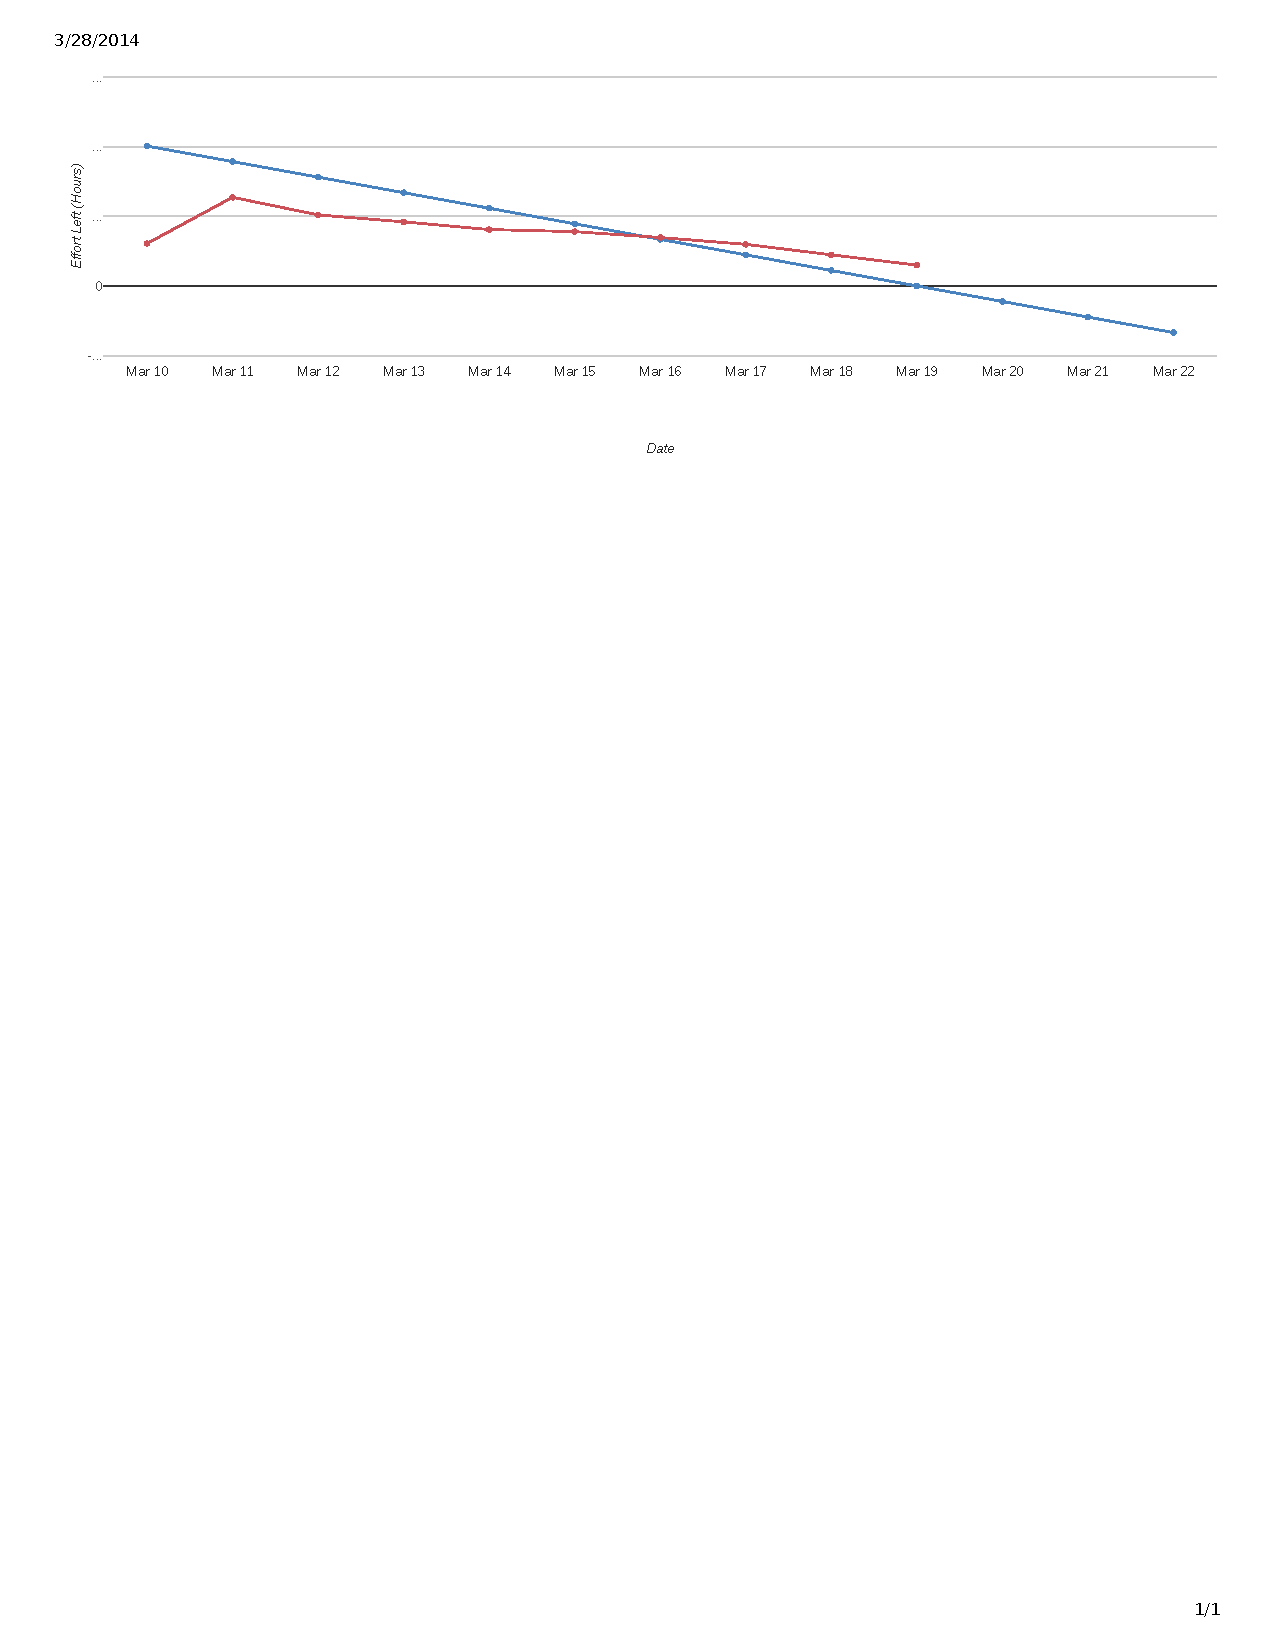
\includegraphics[width=\textwidth, trim= 1cm 21cm 1cm 1cm, clip=true]{ch/projectManagement/fig/burndown4.pdf}
\caption{Sprint 4 burndown chart}
\label{fig:sprint4burndown}
\end{figure}

\subsection{Sprint backlog}

The backlog and time usage result.

\begin{table}[H]
	\begin{tabular}{|l|p{7cm}|p{2.2cm}|p{1.5cm}|p{1.5cm}|}%
		\hline \bfseries User story & \bfseries Details & \bfseries Hours\newline estimated & \bfseries Hours spent & \bfseries Hours left
		\csvreader[head to column names]{ch/projectManagement/sec/sprints/sprint4/userstories.csv}{}% use head of csv as column names
		{\\\hline \id & \title & \estimated & \spent & \left} \\\hline% specify your coloumns here
	\end{tabular}
    \caption{Sprint 4 backlog}
\end{table}

\subsection{Issues and solutions}
Naturally the team ran into a lot of problems with implementation in Android, which was a completely new development environment for half of the team. A team member ran into problems with Facebook authentication in Android due to inexperience and confusing documentation. After this task was recognized as an issue, it was reassigned to a more experienced member in an attempt to maintain the progress of the project. There were also minor problems reaching the development goal for the sprint as the workload for the midterm report delivery was underestimated a bit. This lead to the reallocation of resources from development to documentation, and pushed some user stories to the next sprint.

\subsection{Work completed}
The most important milestone of the sprint was the midterm report that was due for delivery on the last day of the sprint. Other important work was prototyping the different tabs. Facebook login logic was completed and very basic functionality for most tabs was in place at the end of the sprint.

\subsection{Sprint review}
This sprint had two factors that made it into a very productive, but very exhausting sprint for the team members. The previous sprint had not met expectations on completed work and the users stories in the current sprint had been underestimated. This lead to the team working overtime, exceeding the expected working hours by 30 percent. Naturally, the progress was uplifting, but the team was at the same time exhausted from all the extra work. It was decided to up the estimates on the next sprint since it became apparent that estimations so far had been too conservative. The team agreed it would be better to overestimate and add tasks to the sprint rather than underestimate and not finish the goals set in conjunction with the customer.